\documentclass[a4paper]{article}

\usepackage[english]{babel}
\usepackage[utf8]{inputenc}
\usepackage{mathtools}
\usepackage{gensymb}
\usepackage{amssymb}
\usepackage{amsmath}
\usepackage[thmmarks,amsmath]{ntheorem}
\usepackage{booktabs,siunitx}
\usepackage{graphicx}
\usepackage[colorinlistoftodos]{todonotes}
\usepackage{geometry}
\usepackage{float}
\usepackage{hyperref}
\usepackage{caption}
\usepackage[bottom]{footmisc}
\geometry{
 a4paper,
 total={170mm,257mm},
 left=30mm,
 right=30mm,
 top=20mm,
 }
\author{[[Name]]}
\title{Report - [[Experiment]]}

\begin{document}

\maketitle
\abstract 

The appearance of the  Peltier effect can be used to build thermoelectric heat pumps or refrigerators. When two metal rods are connected and a current flows trough, heat generation or cooling occures at their junction; this is called the Peltier effect. In addition to this, there is a temperature gradient inside the rods belonging to Joule heating. In this experiment the relative Peltier coefficient $\Pi_{12}$, which is the amount of heat carried per unit charge, is measured for a copper/constantan rod soldered at their junction. The coefficient is found to be dependent of the temperature at the far ends, but not of the current. It also depends on the materials. The measured values can be found in table \ref{tab:peltierCoeffs}.

\section{Introduction}
\label{sec:introduction}

The Peltier effect is the phenomenon of heat generation or cooling at the junction of two metal conductors when a current is applied trough the element. The far ends of these conductors must be held at a constant temperature. Depending on the sign of the applied current, the junction warms up or cools down (relative to the temperature of the metals). Since the two metals are not the same, at the junction there is a discontinuity in heat flow $\vec{U}$, because the current must be continuous, leading to a heating or cooling the junction. The jump in the discontinuity is proportional to the current density $\vec{J}$ and the relative Peltier coefficient $\Pi_{12}$.
\newline
There is also an amount of heating with is not negligible due to another (well known) effect called Joule heating. This is, when current is applied to a metal conductor, the material dissipates heat, although this effect does not depend on the sign of the current, because it is proportional to the square of the current density $Q_{Joule} \propto \rho \vec{J}^2$.
\newline
The Onsager relation say

\begin{subequations}
\begin{align}
    E &= \rho \vec{J} + \epsilon \nabla T \	\label{eq:E} \\
    U &= \Pi \vec{J} - \kappa \nabla T \ \label{eq:U}
\end{align}
\end{subequations}

Considering the local conservation of heat

\begin{equation}
\frac{du}{dt} = - \nabla \cdot \vec{U} + \vec{J} \cdot \vec{E}
\end{equation}

and setting $\frac{du}{dt} = 0$ in the steady state, one accuires:

\begin{subequations}
\begin{align}
	\nabla \cdot \vec{U} &= \vec{J} \cdot \vec{E} \\
	\nabla \cdot \left( \Pi \vec{J} - \kappa \nabla T \right) &= \vec{J} \cdot \left( \rho \vec{J} + \epsilon \nabla T \right) \ \label{eq:3b} \\
	\nabla \cdot \left( \epsilon T \vec{J} - \kappa \nabla T \right) &= \vec{J} \cdot \left( \rho \vec{J} + \epsilon \nabla T \right) \ \label{eq:3c} \\
	\epsilon T \nabla \vec{J} + \epsilon \left( \nabla T \right) \vec{J} - \kappa \nabla^2 T &= \rho \vec{J}^2 + \epsilon \vec{J} \nabla T \ \label{eq:3d} \\
	\epsilon T \nabla \vec{J} - \kappa \nabla^2 T &= \rho \vec{J}^2 \label{eq:3e} \\
	\kappa \nabla^2 T &= - \rho \vec{J}^2 \ \label{eq:jsquare}
\end{align}
\end{subequations}

Equation \eqref{eq:3b} is obtained after inserting equations \eqref{eq:E} and \eqref{eq:U}. For \eqref{eq:3c} the Onsager relation $\Pi = \epsilon T$ was used. In equation \eqref{eq:3d} the bracket was expanded and the product rule for derivatives was applied. Equation \eqref{eq:3e} is just equation \eqref{eq:3d} simplified. At equilirium the current density $\vec{J}$ is constant in the metal conductor, therefore $\nabla \vec{J} = 0$ and we obtain equation \eqref{eq:jsquare} where we see that Joule heating is proportional to the current density squared, thus depends not on the direction of the current.
\newline
When a current $\pm I$ flows for some time trough the Peltier element, there is a temperature difference between the junction and the oil bath ($\Delta T^{+}$ for positive and $\Delta T^{-}$ for negative current):

\begin{subequations}
\begin{align}
\Delta T^{+} = T_J^{+} - T_b \ \label{eq:deltaTp} \\
\Delta T^{-} = T_b - T_J^{-} \ \label{eq:deltaTp}
\end{align}
\end{subequations}

where $T_J^{\pm}$ is the temperature at the junction for positive and negative current and $T_b$ is the temperature of the oil bath. Integrating \eqref{eq:jsquare} twice in one dimension one obtains a function for $T(x)$:

\begin{subequations}
\begin{align}
T^{''}(x) &= - \frac{\rho \vec{J}^2}{\kappa} \\
\implies T(x) &= -\frac{\rho \vec{J}^2}{2 \kappa} x^2 + T^{'}(0) \, x + const. \\	
\implies \Delta T^{\pm} &= T(0) - T(-L_1) = \frac{\rho_1 L_1^2}{2 \kappa_1 F_1^2} I^2 + L_1 T_1^{\pm'}(0) \ \label{eq:dtpm1} \\
\implies \Delta T^{\pm} &= T(0) - T(L_2) = \frac{\rho_2 L_2^2}{2 \kappa_2 F_2^2} I^2 - L_2 T_2^{\pm'}(0) \ \label{eq:dtpm2}\\
\end{align}
\end{subequations}

These $\Delta T^{\pm}$ are measurable quantities. From equation \eqref{eq:U} we get for $i \in \{1, 2\}$

\begin{subequations}
\begin{align}
U_i(0) &= \frac{\Pi_i I}{F_i} - \kappa_i T_i^{\pm'}(0) \\
\implies \Pi_i I &= F_i U_i(0) + F_i \kappa_i T_i^{\pm'}(0) \\
\implies \pm \Pi_{12} I &= \pm I \left( \Pi_1 - \Pi_2 \right) = F_1 U_1(0) - F_2 U_2(0) + F_1 \kappa_1 T_1^{\pm'}(0) - F_2 \kappa_2 T_2^{\pm'}(0)
\end{align}
\end{subequations}

Where $\Pi_i$ are absolute Peltier coefficients of the corresponding materials $1$ and $2$, and $\Pi_{12}$ is the relative Peltier coefficient of them respectively. In stationary state we have $F_1 U_1(0) = F_2 U_2(0)$ and after inserting equations \eqref{eq:dtpm1} and \eqref{eq:dtpm2} solved for $T_i^{\pm'}(0)$ we get

\begin{equation}
\pm \Pi_{12} I = \left( \frac{\kappa_1 F_1}{L_1} + \frac{\kappa_2 F_2}{L_2} \right) \Delta T^{\pm} - \frac{R_1 + R_2}{2} I^2 \label{eq:pmi}
\end{equation}

with $R_i = \frac{\rho_i L_i}{F_i}$ for $i \in \{1, 2\}$. The equation with $\Delta T^{+}$ can be substracted from the equation with $\Delta T^{-}$ to obtain an equation for the Peltier coefficient. The advantage is that by substracting the two temperature differences Joule heating can be eleminated. By adding them we get a second equation:

\begin{subequations}
\begin{align}
\left( \frac{\kappa_1 F_1}{L_1} + \frac{\kappa_2 F_2}{L_2} \right) \frac{\Delta T^{+} + \Delta T^{-}}{I} = \left( R_1 + R_2 \right) I \approx V_p \ \label{eq:adding}
\end{align}
\end{subequations}

From this equation we can obtain another equation for the Peltier coefficient depending on the Peltier voltage $V_p$. The other one depends on the current $I$.

\begin{subequations}
\begin{align}
\Pi_{12}^{(V)} &= \frac{V_p}{2} \frac{\Delta T^{+} - \Delta T^{-}}{\Delta T^{+} + \Delta T^{-}} \ \label{eq:pi12v} \\
\Pi_{12}^{(I)} &= \left( \frac{\kappa_1 F_1}{L_1} + \frac{\kappa_2 F_2}{L_2} \right) \frac{\Delta T^{+} - \Delta T^{-}}{2 I} \ \label{eq:pi12i}
\end{align}
\end{subequations}

These are the two elementary equations needed to calculate the relative Peltier coefficient of two metal conductors only from measurable quantities.

\section{Setup}

The heart piece of the experiment is the Peltier element. A copper/constantant rod was used. The constantan part consisted of an alloy of $45\%$ nickel and $55\%$ copper. The copper and constantan were soldered at their junction. The other ends were connected to copper blocks which were held at a constant temperature $T_b$. These copper blocks were immersed in an oil bath, whereas the Peltier element was in a diving bell filled with air and thus had no direct contact to the oil bath. A magnetic stirrer was used to circulate the oil to achieve a minimisation of the temperature gradient across the oil bath. A heater was connected to the oil bath. Sensing wires from the copper blocks were connected to a voltage meter to measure the Peltier voltage $V_p$. Another set of sensing wires were conected to the Peltier elements junction and to the upper connection between the Peltier element and the copper block to measure the voltage difference $V_T$ (see figure \ref{fig:setup}). From the voltage difference $V_T$ the temperature difference $\Delta T$ can be calculated using the reference table of the thermocouple.

\begin{figure}[H]
\captionsetup{singlelinecheck=off}
\centering
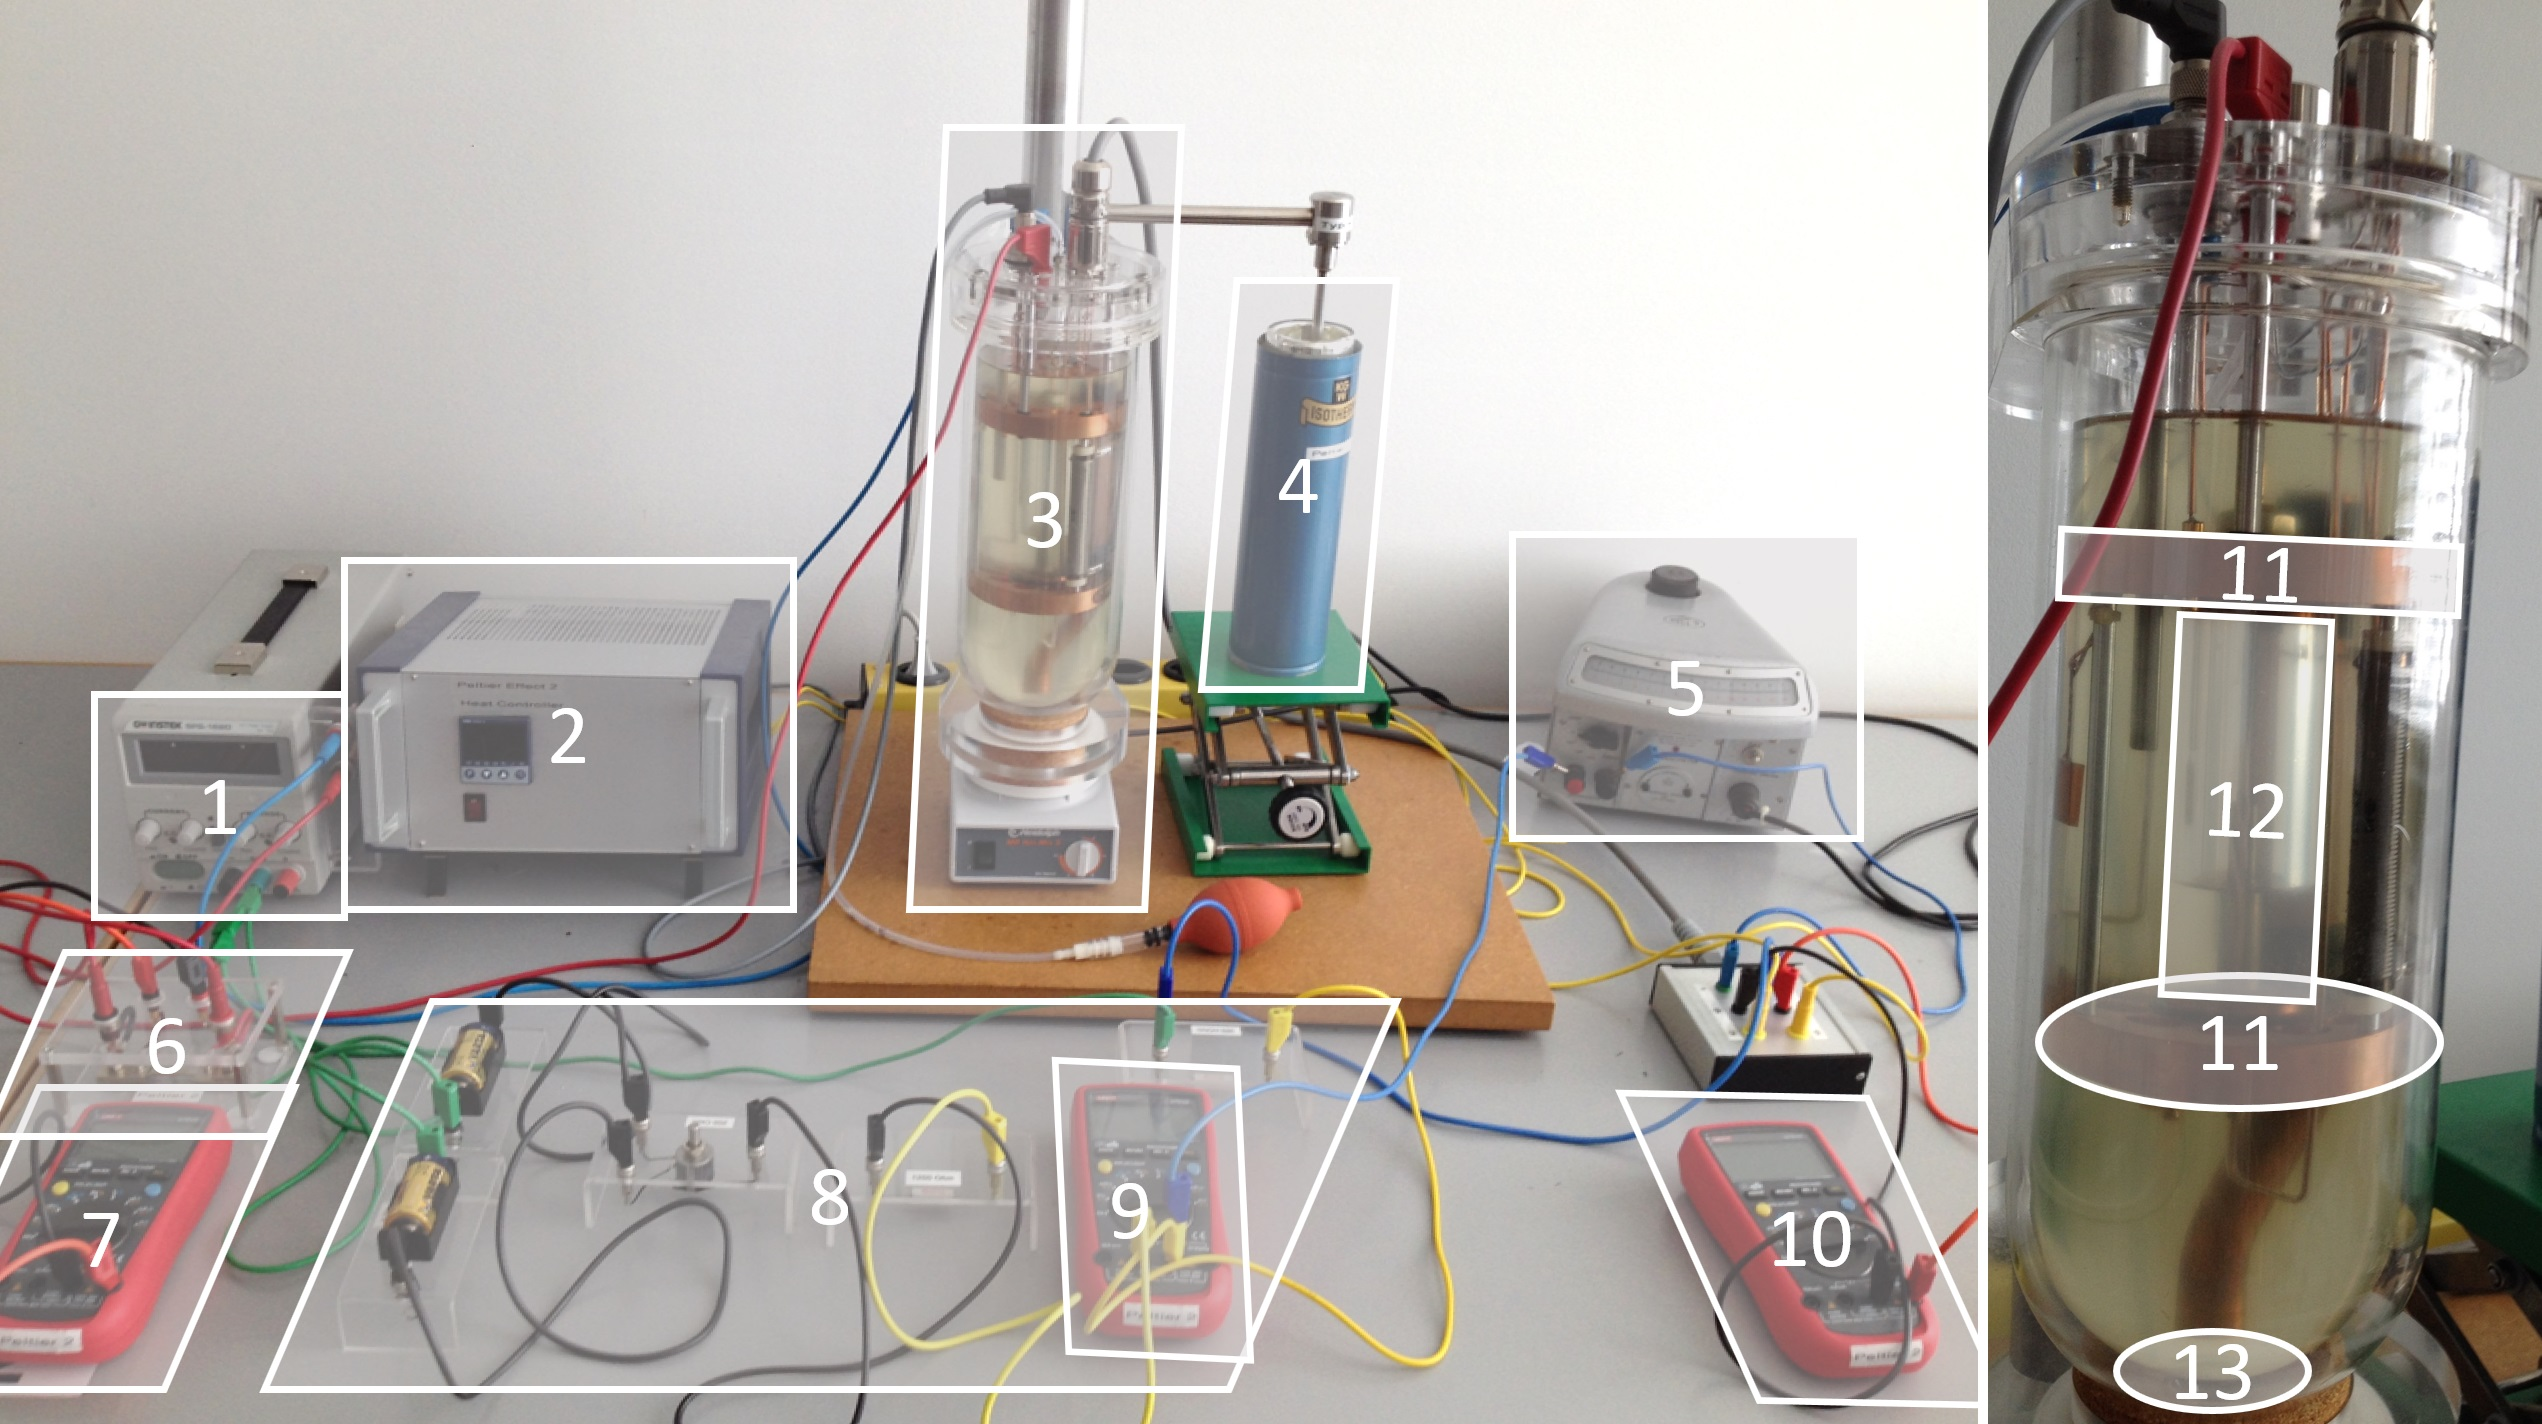
\includegraphics[width=1.0\textwidth]{img/setup.jpg}
\caption[blubb]{Image of the experimental setup. $1$ is the power supply, $2$ the heater, $3$ the oil bath with the Peltier element, $4$ is the ice bath, $5$ the galvanometer used in the compensation circuit, $6$ the shunt resistor with the voltage meter $7$ which measures $V_S$, $8$ is the compensation circuit with the two $1.5 \, V$ batteries, the potientiometer, the two resistors and $9$ the ammeter to measure $I_T$, $10$ is the voltmeter to measure the Peltier voltage $V_p$. On the right side, a closer look at the oil bath with the copper-constantan rods is depicted. $11$ are the copper blocks immersed in oil, $12$ is the Peltier element (in the image can be seen that oil leaks in the area of the two conductors (see section \ref{sec:systematic_errors})), $13$ is the magnetic stirrer. Source: Authors' own.}
\label{fig:setup}
\end{figure}

Aside the oil bath, a cooling bath of ice and water was held at reference temperature $0^{\circ}C$. The connections of the sensing wires for $V_T$ were immersed in the cooling bath, such that the surrounding temperature was around $0^{\circ}C$. Because of that, the temperatures in the reference table \cite{thermocouple} of the thermocouple could be seen as absolute, instead of relative temperatures.
\newline
A constant current $I$ flew from the one to the other copper block, thus trough the Peltier element and caused the element to heat or cool. The power supply was in series with a shunt resistor over which the voltage $V_S$ dropped, providing a stable current.
\newline
The quantities $V_p$ and $V_T$ were measured for different temperatures $T_b$ ($30^{\circ}C, 50^{\circ}C, 80^{\circ}C, 110^{\circ}C$) and currents $I$ ($\pm 4 \, A, \pm 8 \, A, \pm 12 \, A, \pm 16 \, A$).

\section{Measurement Method}

Since the Peltier coefficient is proportional to the difference in voltage of the two metals and inverse proportional to the electric current density $\vec{J}$, we cannot measure it directly. It must be calculated from of measurable quantities.
\newline
The voltage difference between the junction of the two metals and the oil bath $V_T$ can be measured with a type-K thermocouple. From this, with the usage of its reference table \cite{thermocouple}, we obtain the difference in temperature $\Delta T = T_{b} - T_J$ where $T_b$ is the temperature of the oil bath and $T_J$ the temperature at the junction of the two metals.
\newline
The voltage difference between the upper and the lower end of the Peltier element $V_p$ can be measured too.
\newline
With those 3 values ($V_T$, $V_p$ and $I$), we can calculate the Peltier coefficient according to the theory in 2 ways (equations \eqref{eq:pi12i} and \eqref{eq:pi12v}).

\subsection{Measuring $I$}

For the measurement of the incoming current $I$ a shunt resistor was used because the device supplying the current was not reliable in regulating and reading off the current precisely enough. The voltage over the shunt was measured as $V_S$ with a multimeter connected over the shunt. With that value, the real value of the current was calculated using the properties of the shunt itself ($I_{Shunt} = [[I_Shunt]]\, A$ and $V_{Shunt} = [[V_Shunt]]\, mV$) with the URI-formula:

\begin{equation}
I = \frac{V_S}{R_{Shunt}} = \frac{V_S \cdot I_{Shunt}}{V_{Shunt}}
\label{eq:current}
\end{equation}

\subsection{Measuring $V_p$}

The measurement of $V_p$ was straightforward. A multimeter was connected to the corresponding connectors, given in the experiment installation. These two connectors lead to the upper and the lower end of the Peltier element.

\subsection{Measuring $V_T$}

Since $V_T$ is in the regime of $\mu V$, the resistance of the cables and contact is not negligible anymore. A compensation circuit was used to measure it (see figure \ref{fig:cc}).

\begin{figure}[H]
\captionsetup{singlelinecheck=off}
\centering
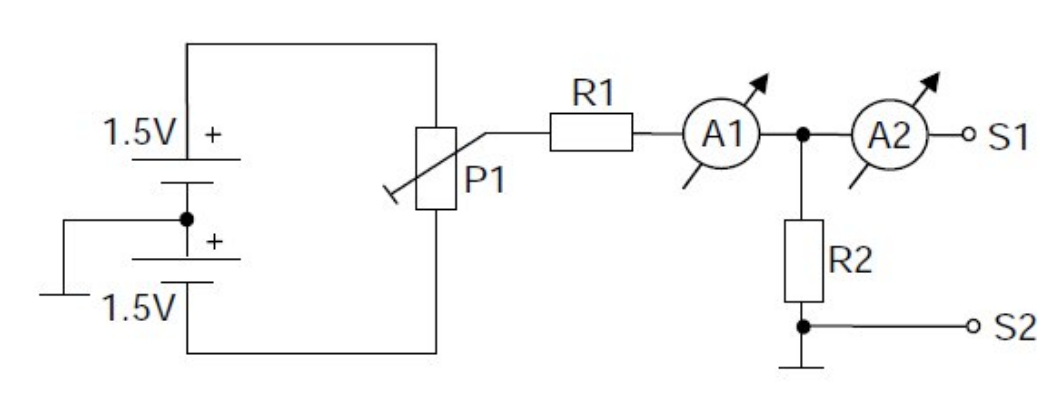
\includegraphics[width=0.8\textwidth]{img/compensation_circuit.png}
\caption[blubb]{Compensation circuit. Source: Instruction Sheet.}
\label{fig:cc}
\end{figure}

In this circuit the value of $I_T$ is measured with a multimeter ($A1$). To measure a value of $I_T$ the potentiometer ($P1$) was adjusted until no current flew trough the galvanometer ($A2$). $S1$ and $S2$ were connected to the Peltier element to measure $V_T$. With $I_T$ given, $V_T$ can be calculated using

\begin{equation}
V_T = R_2 \cdot I_T
\label{eq:V_T}
\end{equation}

The value of $R_2$ in the compensation circuit was given in the instruction sheet as $R_2 = [[R_2]]\, m\Omega$. Usually the value of $I_T$ was in the regime of $\mu A$.

\subsection{Calculating $\Delta T^{\pm}$}

To obtain the temperature difference between the junction and the upper end of the Peltier element $\Delta T^{\pm}$, the reference table of the type K thermocouple was used. For this, the part of the table containing the relevant temperature differences ($-10^{\circ}C$ to $10^{\circ}C$) was interpolated to a linear fit line:

\begin{equation}
f(V_T) = [[thermoFitline]]
\label{eq:thermoFitline}
\end{equation}

\subsection{Calculating the Peltier coefficient}

Given the temperature difference $\Delta T^{\pm}$ for $\pm I$, the Peltier coefficient was calculated using both of the formulas (\eqref{eq:pi12i} and \eqref{eq:pi12v}) stated in section \ref{sec:introduction}.

\newpage
\section{Measurements}

The measured values used and discussed in this report can be found in the following tables (table \ref{tab:measure30}, \ref{tab:measure50}, \ref{tab:measure80} and \ref{tab:measure110} for the measurements of temperature $30^{\circ}C$, $50^{\circ}C$, $80^{\circ}C$ and $110^{\circ}C$ respectively). The values for the current $I$ and the calculations for the $\Delta T^{\pm}$ are also given on the tables for overview. Notice that not each measurement (even of the same quantity) has the same number of significant figures (see for example the column for $I_T$ in table \ref{tab:measure30}). This is due to the multimeter used to measure, changing the range of measurement automatically and thus the significant figures of the value.

The calculated values for the Peltier coefficients to a given temperature $T_b$ and current $I$ are in the following tables (table \ref{tab:pi12i} and \ref{tab:pi12v}).

\begin{table}[H]
\centering
\begin{tabular}{r|rrrr}
[[Pi12VTable]]
\end{tabular}
\caption{Calculated Peltier coefficients $\Pi_{12}^{(V)}$.}
\label{tab:pi12v}
\end{table}

\begin{table}[H]
\centering
\begin{tabular}{r|rrrr}
[[Pi12ITable]]
\end{tabular}
\caption{Calculated Peltier coefficients $\Pi_{12}^{(I)}$.}
\label{tab:pi12i}
\end{table}

\subsection{Errors}

The error of $I_T$ was cumbersome to estimate. It was chosen to be the change in the measured value of $I_T$ of one section in the scale of the galvanometer (see figure \ref{fig:scale}). When the system was in equilibrium and the potentiometer was adjusted, such that the the galvanometer displayed zero, the value of $I_T$ was measured to be $a$. Then we adjusted the potentiometer until the pointer of the galvanometer was one line to the right. After that, $I_T$ was measured to be $b$. The error of $I_T$ was then calculated to be $\Delta I_T = |a-b| + \Delta c$ where $\Delta c$ is the error of the multimeter. The value of $|a-b|$ was measured $[[deltaScale]] A$. The multimeter used was a UNI-T UT61C \cite{multimeter}. In the manual, the error for ampere measurements in the $\mu A$ range is decalred [[deltaMMA]]. So the total error of one measurement of $I_T$ is [[deltaI_T_tot]].

\begin{figure}[H]
\captionsetup{singlelinecheck=off}
\centering
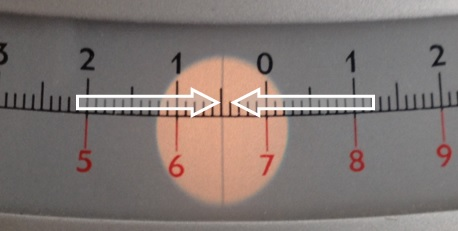
\includegraphics[width=0.6\textwidth]{img/scale.jpg}
\caption[blubb]{Illustration of exactly one unit in the scale of the galvanometer. Source: Authors' own.}
\label{fig:scale}
\end{figure}

For the measurement of $V_S$ and $V_p$ the same type of multimeter was used. In the manual, the error for voltage measurements in the $mV$ range was declared as [[deltaMMV]].
\newline
To calculate the current $I$ from equation \eqref{eq:current}, no error estimations for $V_{Shunt}$ and $I_{Shunt}$ were given on the instruction sheet. Therefore these two values were supposed to be analytically exact and thus don't provide input to the error propagation.

\newpage
\section{Discussion}

In order to evaluate the quality of the measurements, the following three plots and their functional dependance are discussed.

\subsection{Plot of $\Delta T^{\pm}$ against $I$}

In figure \ref{fig:dtpmvsi} the calculated points of the temperature differences $\Delta T^{\pm}$ are plotted against the currents $I$.

\begin{figure}[H]
\captionsetup{singlelinecheck=off}
\centering
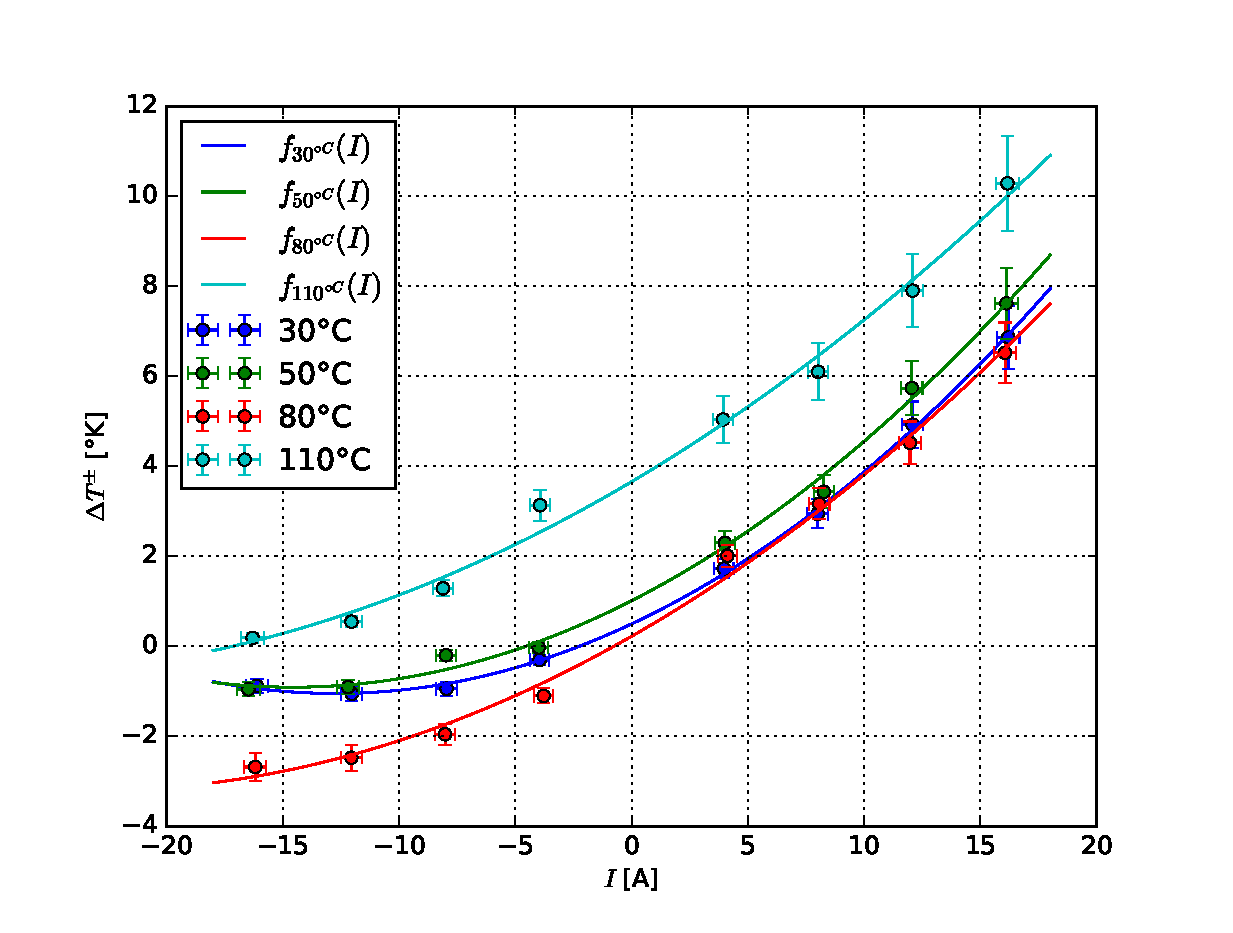
\includegraphics[width=0.6\textwidth]{plots/dT_vs_I.eps}
\caption[blubb]{Plot of $\Delta T^{\pm}$ against $I$ with their quadratic fit. These are as follows:
\begin{itemize}
\item $f_{30^{\circ}C}(I) = [[dtpmfit30]]$
\item $f_{50^{\circ}C}(I) = [[dtpmfit50]]$
\item $f_{80^{\circ}C}(I) = [[dtpmfit80]]$
\item $f_{110^{\circ}C}(I) = [[dtpmfit110]]$
\end{itemize} Source: Authors' own.}
\label{fig:dtpmvsi}
\end{figure}

From equations \eqref{eq:dtpm1} and \eqref{eq:dtpm2} can be seen that the $\Delta T^{\pm}$ depend on $I^2$. The corrensponding quadratic polynomial fits are plotted in the figure too. The calculated points of $\Delta T^{\pm}$ correspond quite well to the theory. The fact that the temperature differences for negative currents are smaller in magnitude than the differences of the positive currents makes sense. This is due to the reason that Joule heating is always positive (see equation \eqref{eq:jsquare}) following that positive temperature differences are to high and negative are to low in magnitude.
\newline
It is notable that the points for $T_b = 110^{\circ}C$ are all positive whereas for the other temperatures there are 4 negatve and 4 positive points. Thus even the values for $\Delta T^{-}$ are positive in this case (see table \ref{tab:measure110}). An explanation for this could be that for $T_b = 110^{\circ}C$ the heating coming from Joule heating is greather than the cooling effect of Peltier heating, resulting in a positive temperature difference.

\newpage
\subsection{Plot of $\Delta T^{+} + \Delta T^{-}$ against $I$}

Figure \ref{fig:dtppdtm} illustrates the functional dependence of the addition of the temperature differences for positive and negative currents $\Delta T^{+} + \Delta T^{-}$ from the mean current $I$ in magnitude.

\begin{figure}[H]
\captionsetup{singlelinecheck=off}
\centering
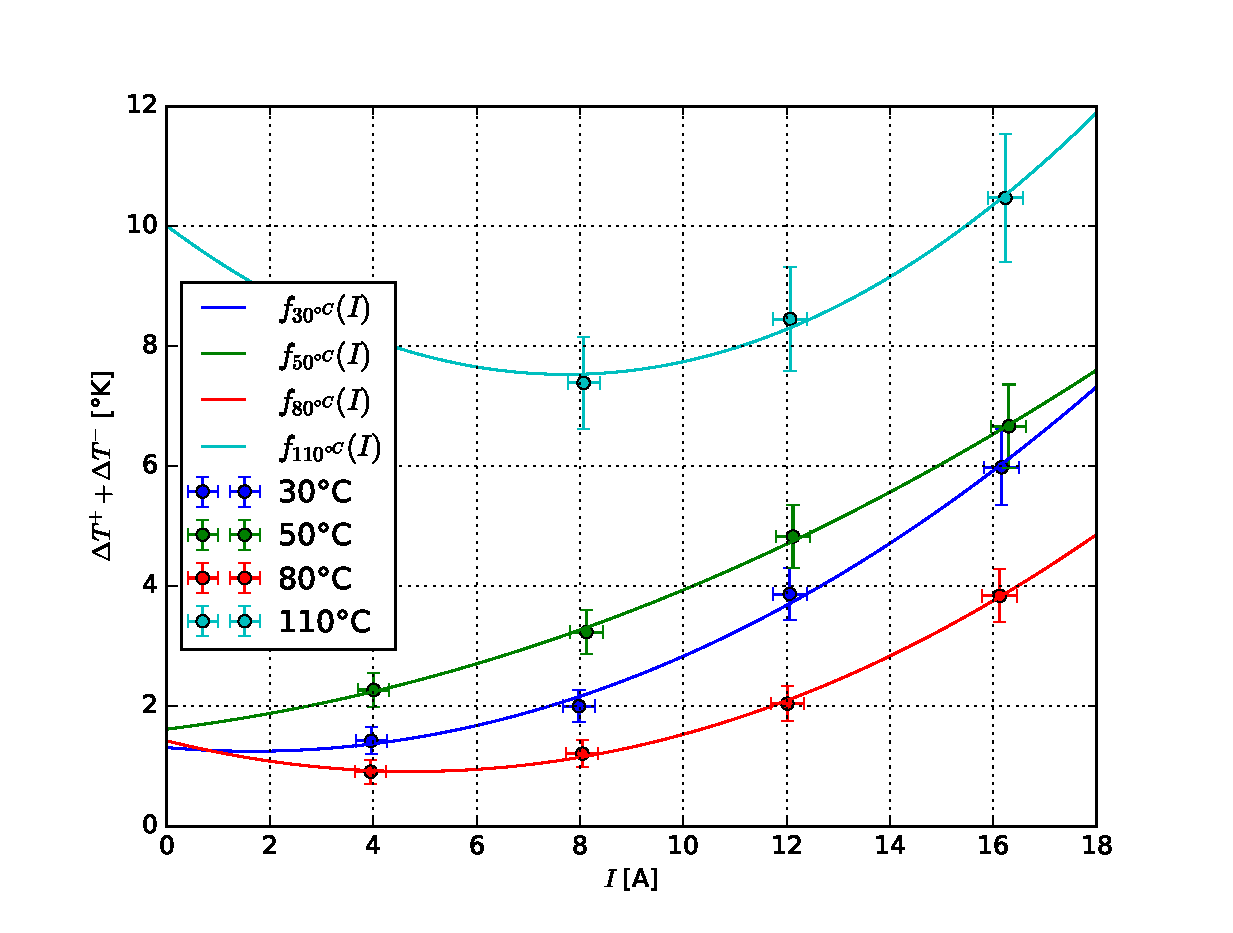
\includegraphics[width=0.6\textwidth]{plots/dTp+dTm_vs_I.eps}
\caption[blubb]{Plot of $\Delta T^{+} + \Delta T^{-}$ against $I$ with their quadratic fits. These are as follows:
\begin{itemize}
\item $f_{30^{\circ}C}(I) = [[dtppdtmfit30]]$
\item $f_{50^{\circ}C}(I) = [[dtppdtmfit50]]$
\item $f_{80^{\circ}C}(I) = [[dtppdtmfit80]]$
\item $f_{110^{\circ}C}(I) = [[dtppdtmfit110]]$
\end{itemize} Source: Authors' own.}
\label{fig:dtppdtm}
\end{figure}

Resolving equation \eqref{eq:adding} for $\Delta T^{+} + \Delta T^{-}$ one gets

\begin{equation}
\Delta T^{+} + \Delta T^{-} = \frac{R_1 + R_2}{\left( \frac{\kappa_1 F_1}{L_1} + \frac{\kappa_2 F_2}{L_2} \right)} I^2 = C_1 I^2
\label{eq:dtppdtm}
\end{equation}

where $C_1$ is just a constant depending on resistor values and the geometry of the experiment. The figure argrees with the theory here, since the calculated points lie on a quadratic polynomial fit in the current $I$. From equation \eqref{eq:dtppdtm} can also be seen that the fits should go trough $0$ for $I=0$. This is approximately the case for all measurements except the one for $T_b = 110^{\circ}C$.

\newpage
\subsection{Plot of $\Delta T^{+} - \Delta T^{-}$ against $I$}

The functional dependence of the difference of the temperature differences for positive and negative currents $\Delta T^{+} - \Delta T^{-}$ from the mean current in magnitude $I$ is displayed in figure \ref{fig:dtpmdtm}.

\begin{figure}[H]
\captionsetup{singlelinecheck=off}
\centering
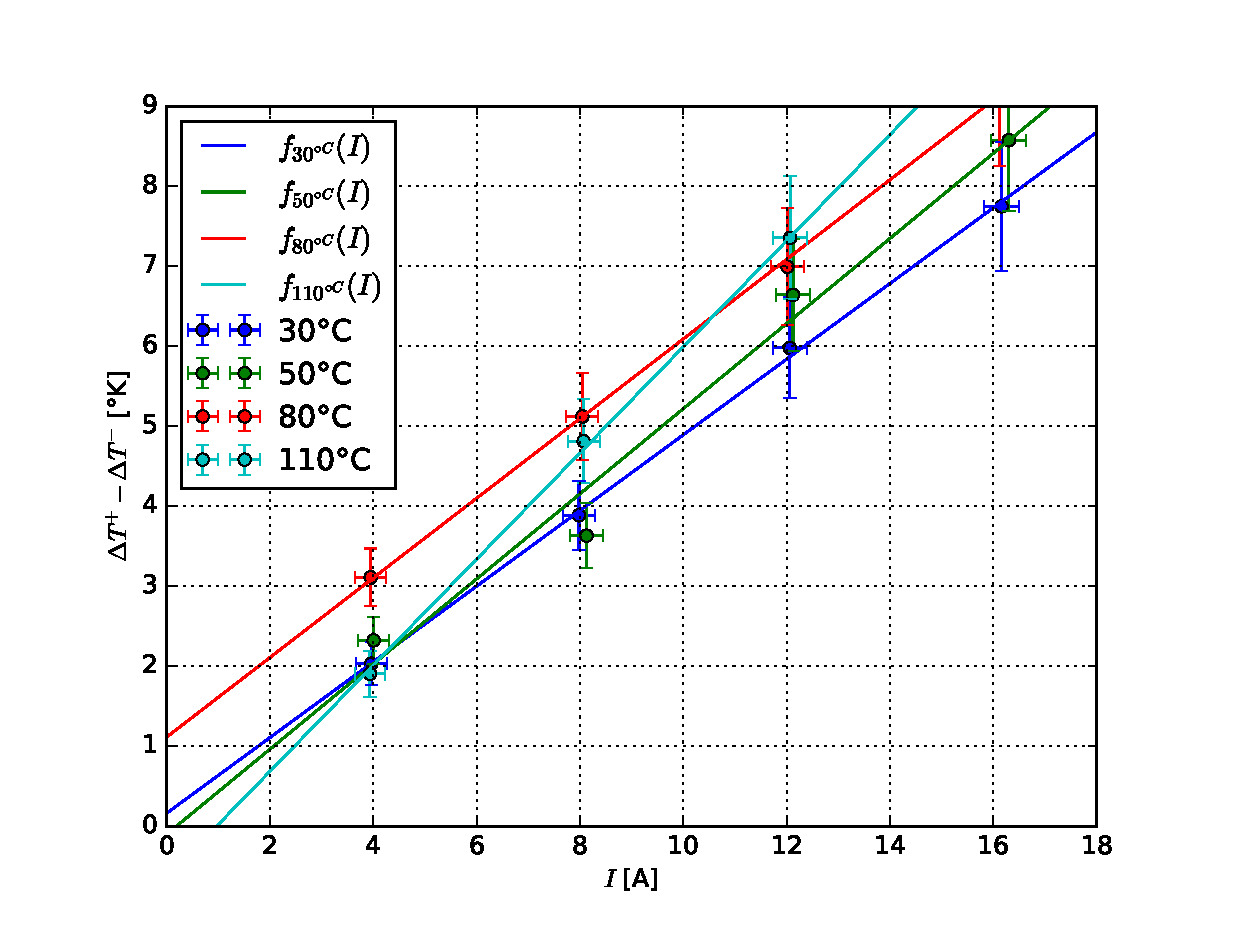
\includegraphics[width=0.6\textwidth]{plots/dTp-dTm_vs_I.eps}
\caption[blubb]{Plot of $\Delta T^{+} - \Delta T^{-}$ against $I$ with their linear fit lines. These are as follows:
\begin{itemize}
\item $f_{30^{\circ}C}(I) = [[dtpmdtmfit30]]$
\item $f_{50^{\circ}C}(I) = [[dtpmdtmfit50]]$
\item $f_{80^{\circ}C}(I) = [[dtpmdtmfit80]]$
\item $f_{110^{\circ}C}(I) = [[dtpmdtmfit110]]$
\end{itemize} Source: Authors' own.}
\label{fig:dtpmdtm}
\end{figure}

From equation \eqref{eq:dtppdtm} we know that $\Delta T^{+} + \Delta T^{-}$ depends quadratic on $I$. Using equation \eqref{eq:pi12v} for $\Pi_{12}^{(V)}$ solved for $\Delta T^{+} - \Delta T^{-}$ and using $V_p \propto I$ from equation \eqref{eq:adding}, one gets

\begin{equation}
\Delta T^{+} - \Delta T^{-} \overset{\text{\ref{eq:pi12v}}}{=} \frac{2 \Pi_{12}^{(V)}}{V_p} \left( \Delta T^{+} + \Delta T^{-} \right) \overset{\text{\ref{eq:dtppdtm}}}{=} \frac{2 \Pi_{12}^{(V)}}{V_p} C_1 I^2 \overset{\text{\ref{eq:adding}}}{=} \frac{2 \Pi_{12}^{(V)}}{ \left( R_1 + R_2 \right) I } C_1 I^2 = C_2 I
\label{eq:dtpmdtm}
\end{equation}

where $C_2$ is another constant depending on the Peltier coefficient (which should be constant in $I$), the resistor values and the geometry of the experiment. Therefore $\Delta T^{+} - \Delta T^{-}$ depends linearly on $I$ and should be $0$ if $I=0$. The measured data and their polynomial fits obey the theory as well.

\subsection{The Peltier coefficient}

According to the theory the Peltier coefficient should not depend on the current, but on the temperature. The mean values across the different currents ($-16 \, A$ to $16 \, A$) were taken for each temperature. The result for every measured temperature can be seen in table \ref{tab:peltierCoeffs}.

\begin{table}[H]
\centering
\begin{tabular}{r|rr|r}
\hline
[[PeltierTable]]
\end{tabular}
\caption{Calculated means over the current $I$ of the Peltier coefficients $\Pi$ in temperature $T_b$.}
\label{tab:peltierCoeffs}
\end{table}

Figure \ref{fig:pivst} shows the mean Peltier coefficients $\Pi_{12}$ taken from both calculations $\Pi_{12}^{(V)}$ and $\Pi_{12}^{(I)}$ plotted against the temperature $T_b$. The literature value is a function $\epsilon(T)$ \cite{bentley98} and \cite{guan2013} where $\epsilon$ is the Seebeck coefficient and $T$ the temperature. The Seebeck and the Peltier coefficient relate, according to the Onsager relations as $\Pi(T) = \epsilon(T) T$.

\begin{figure}[H]
\centering
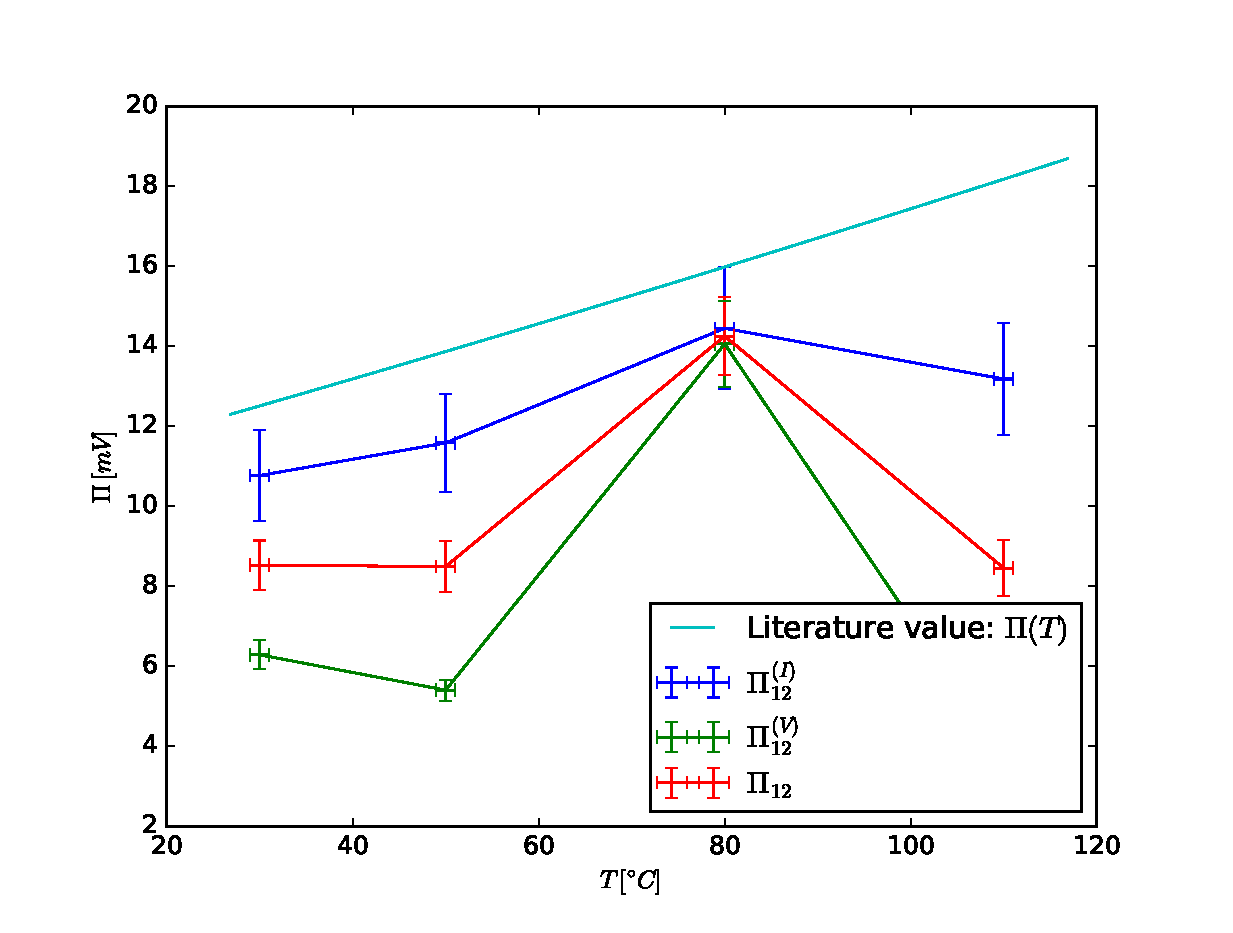
\includegraphics[width=0.6\textwidth]{plots/Pi_vs_T.eps}
\caption{Plot of $\Pi$ against $T_b$. Source: Authors' own.}
\label{fig:pivst}
\end{figure}

The measurements seem to have the same trend as the literature value, except for the measurement of $T_b = 110^{\circ}C$.
\newline
Figure \ref{fig:pi12ivsi} shows the Peltier coefficient $\Pi_{12}^{(I)}$ calculated with formula \eqref{eq:pi12i} against the current $I$.

\begin{figure}[H]
\centering
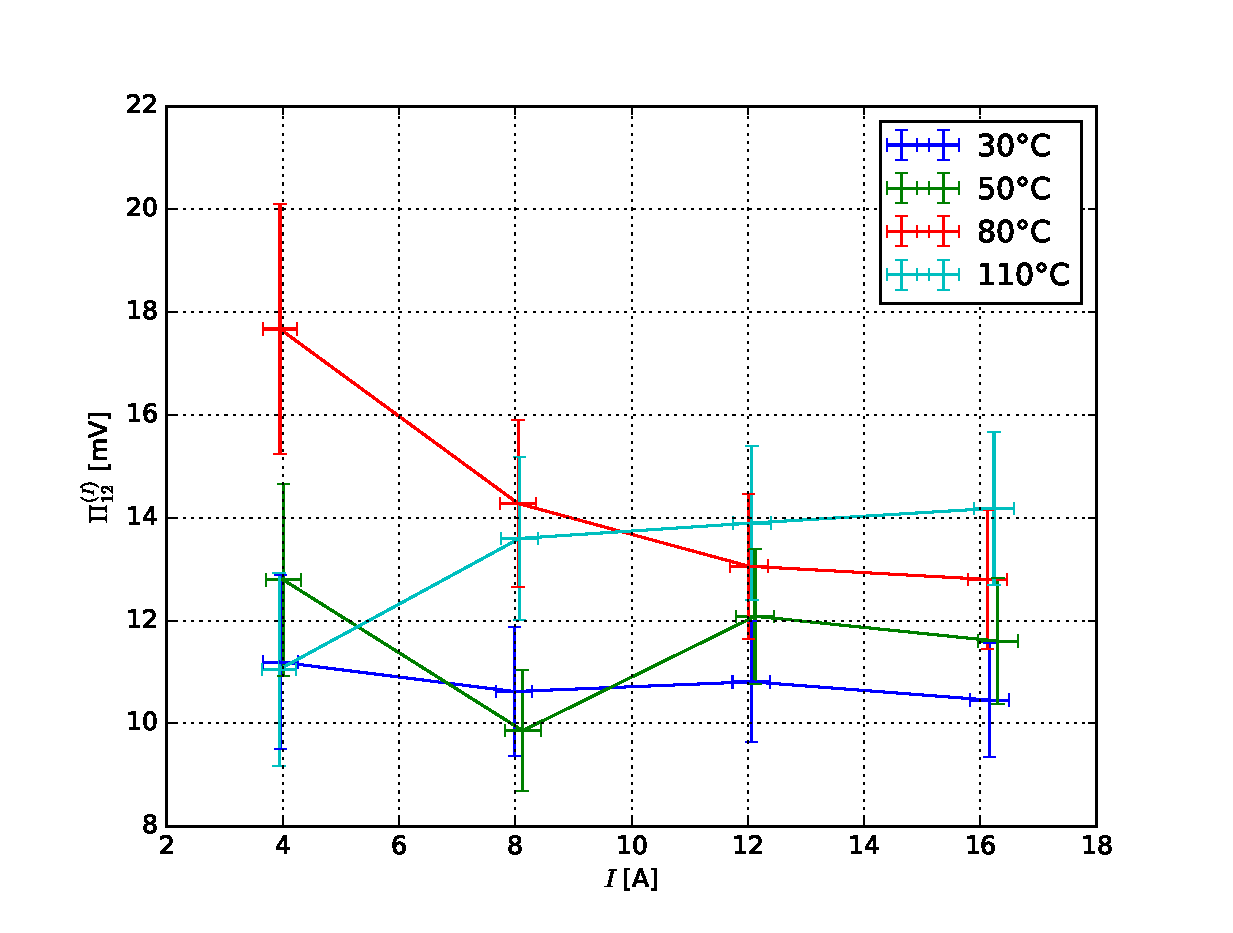
\includegraphics[width=0.6\textwidth]{plots/Pi12I_vs_I.eps}
\caption{Plot of $\Pi_{12}^{(I)}$ against $I$. Source: Authors' own.}
\label{fig:pi12ivsi}
\end{figure}

According to equation \eqref{eq:pi12i} and \eqref{eq:dtpmdtm}, we find

\begin{equation}
\Pi_{12}^{(I)} \overset{\text{\ref{eq:pi12i}}}{=} \left( \frac{\kappa_1 F_1}{L_1} + \frac{\kappa_2 F_2}{L_2} \right) \frac{\Delta T^{+} - \Delta T^{-}}{2 I} \overset{\text{\ref{eq:dtpmdtm}}}{=} \left( \frac{\kappa_1 F_1}{L_1} + \frac{\kappa_2 F_2}{L_2} \right) \frac{C_2 I}{2 I} = C_3
\end{equation}

Therefore the Peltier coefficient does not depend on the current.
\newline
Figure \ref{fig:pi12vvsi} shows the Peltier coefficient $\Pi_{12}^{(V)}$ calculated with formula \eqref{eq:pi12v} against the current $I$.

\begin{figure}[H]
\centering
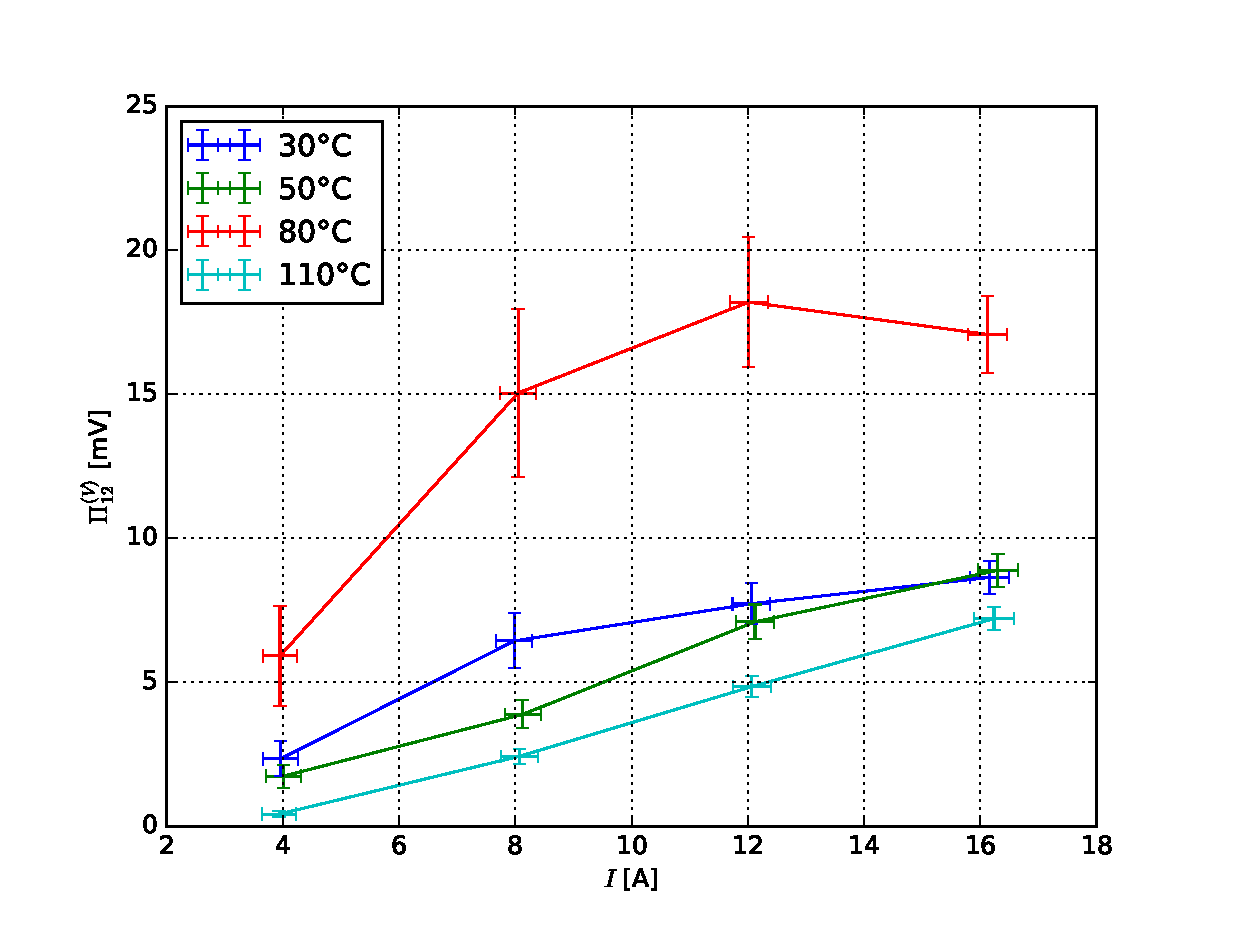
\includegraphics[width=0.6\textwidth]{plots/Pi12V_vs_I.eps}
\caption{Plot of $\Pi_{12}^{(V)}$ against $I$. Source: Authors' own.}
\label{fig:pi12vvsi}
\end{figure}

In a similar manner as above, we can derive that the Peltier coefficient does not depend on the current:

\begin{equation}
\Pi_{12}^{(V)} \overset{\text{\ref{eq:pi12v}}}{=} \frac{V_p}{2} \frac{\Delta T^{+} - \Delta T^{-}}{\Delta T^{+} + \Delta T^{-}} \overset{\text{\ref{eq:dtpmdtm}}}{=} \frac{V_p}{2} \frac{C_2 I}{\Delta T^{+} + \Delta T^{-}} \overset{\text{\ref{eq:dtppdtm}}}{=} \frac{V_p}{2} \frac{C_2 I}{C_1 I^2} \overset{\text{\ref{eq:adding}}}{=} \frac{\left( R_1 + R_2 \right) I}{2} \frac{C_2 I}{C_1 I^2} = C_4
\end{equation}

\subsection{Systematic error sources}
\label{sec:systematic_errors}

In this experiment there are some sources of systematic errors that were ignored. Oil was slowly leaking into the area where the Peltier element was mounted, when the temperature was high ($80^{\circ}C$ and $110^{\circ}C$). This leads to a small systematic error since the temperature gradient was slightly altered. The reference temperature (see figure \ref{fig:setup} label $4$) was assumed to be exact $0^{\circ}C$. This leads to errors in the $\Delta T^{\pm}$. The batteries in the compensation circuit were not exactly $1.5 V$, however this should not be a problem since the compensation circuit stays functional, since the deviation was small. Waiting for convergence of the currrent trough the compensation circuit, lead to small oscillations around a value. Waiting took not seldom more than 20-30 minutes. The value taken for the measurement was the value of $I_T$ after ca. 30 minutes. This leads to a systematic error in $I_T$. There was an unavoidable temperature gradient in the oil bath, leading to a systematic error in $T_b$. At last, when equation \eqref{eq:pi12i} is obtained trough equation \eqref{eq:adding}, resistances in the cables were neglected. This leads to a small systematic error in the measurement of $V_p$.

\subsection{Alternate measurements}

The above analysis of the measured data, suggests that with the measurement for $T_b = 110^{\circ}C$ there is something wrong. We took the measurements for $110^{\circ}C$ twice. The alternative measurements can be found in table \ref{tab:measure1102}. These were not taken in the discussion, because the authors adjudged that the current $I_T$ was not converged already. In the second measurement (the one that was taken), we waited around 30-40 minutes for the current to converge.

\subsection{Conclusion}

The calculated mean values for the Peltier coefficient (see table \ref{tab:peltierCoeffs}) agree mostly with the literature values (see figure \ref{fig:pivst} and reference \cite{guan2013}), except for the measurements with $T_b = 110^{\circ}C$. There might be a systematic error occured during the experiment. 
\newline
Also a reasonable suspicion was that we waited not long enough for convergence of the current $I_T$ in the measurement for $T_b = 110^{\circ}C$. When repeatng the experiment, the autor highly recommends to wait longer (at least 1 hour) for the convergence of the current $I_T$ trough the compensation circuit. Since this has to be done for every single measurement, it will take long measure time to perform the whole experiment.
\newline
The examination of thermoelectric effects, such as the Peltier or the Seebeck effect are important in material sciences. The Peltier effect has a significant role when it comes to efficiency and power consumption of thermoelectric heat pumps and cooling devices such as refrigerators \cite{wiki2018}.

\begin{thebibliography}{9}

\bibitem{bentley98}
  R. E. Bentley,
  \textit{Theory and Practice of Thermoelectric Thermometry (Handbook of Temperature Measurement Vol. 3)},
  Springer-Verlag, Singapore,
  p. 27,
  1998.

\bibitem{guan2013}
  Guan, Aiqiang  and Wang,Hanfu  and Jin,Hao  and Chu,Weiguo  and Guo,Yanjun  and Lu,Guiwu,
  \textit{An experimental apparatus for simultaneously measuring Seebeck coefficient and electrical resistivity from 100 K to 600 K},
  Review of Scientific Instruments,
  p. 5,
  doi: 10.1063/1.4798647,
  2013.

\bibitem{thermocouple}
  NIST,
  \textit{ITS-90 Thermocouple Database [Online]},
  October 20, 2018,
  \url{https://srdata.nist.gov/its90/main/},

\bibitem{multimeter}
  UNI-T, UT61C Multimeter [Online],
  \textit{UNI-T UT61C Multimeter},
  October 20, 2018,
  \url{http://uni-trend.com/productsdetail.aspx?ProductsID=603&ProductsCateId=743&CateId=743},

\bibitem{wiki2018}
  Wikidpedia, [Online],
  \textit{Thermoelectric effect},
  October 21, 2018,
  \url{https://en.wikipedia.org/wiki/Thermoelectric_effect#Peltier_effect},

\end{thebibliography}

\newpage

\section{Appendix}

All measured data that was used in the calculation in the report can be found in the tables underneath.
\newline

\begin{table}[H]
\centering
\begin{tabular}{r|rrrr}
\hline
[[table30]]
\end{tabular}
\caption{Measured data for $T=30^\circ\text{C}$.}
\label{tab:measure30}
\end{table}

\begin{table}[H]
\centering
\begin{tabular}{r|rrrr}
\hline
[[table50]]
\end{tabular}
\caption{Measured data for $T=50^\circ\text{C}$.}
\label{tab:measure50}
\end{table}

\begin{table}[H]
\centering
\begin{tabular}{r|rrrr}
\hline
[[table80]]
\end{tabular}
\caption{Measured data for $T=80^\circ\text{C}$.}
\label{tab:measure80}
\end{table}

\begin{table}[H]
\centering
\begin{tabular}{r|rrrr}
\hline
[[table110]]
\end{tabular}
\caption{Measured data for $T=110^\circ\text{C}$.}
\label{tab:measure110}
\end{table}

All additional measured data can be found in the tables underneath.
\newline

\begin{table}[H]
\centering
\begin{tabular}{r|rrrr}
\hline
[[table1102]]
\end{tabular}
\caption{Alternate measured data for $T=110^\circ\text{C}$.}
\label{tab:measure1102}
\end{table}

\begin{table}[H]
\centering
\begin{tabular}{r|rrrr}
\hline
[[table802]]
\end{tabular}
\caption{Alternate measured data for $T=80^\circ\text{C}$.}
\label{tab:measure1102}
\end{table}

\end{document}

